\documentclass{article}
\usepackage{amsmath}
\usepackage{hyperref}
\usepackage{graphicx}
\usepackage{amssymb}
\setlength\parindent{0pt}
\title{Optical Fiber Geophysics HW 1}
\date{10/07/2022}
\author{Simon Hans Edasi}
\begin{document}
	\maketitle
	
	
\section{Ampere's Law}

Start with Ampere's Law and constitutive relations as given in lecture:

\begin{align}
\vec{\nabla} \times \vec{H} = \vec{J} + \frac{\partial \vec{D}} {\partial t};
\qquad
\vec{J} = \sigma \vec{E};
\qquad
\vec{D} = \epsilon_{0} \vec{E} + \epsilon_{0} \chi_{e} \vec{E} = \epsilon \vec{E}; \quad \epsilon = \epsilon_{0}(1+\chi_{e})
\end{align}


Use constitutive relations to rewrite in terms of $\vec{E}$.

\begin{align}
\vec{\nabla} \times \vec{H} = \sigma \vec{E} + \epsilon \frac{\partial}{\partial t} \vec{E}
\end{align}



Stokes' Theorem allows us to integrate a curl of $\vec{H}$ as a surface integral of $\vec{H}$. We can thus write Ampere's law as:


\begin{align}
\oint \left( \vec{\nabla} \times \vec{H} \right) \cdot dl = \iint \left( \sigma \vec{E} + \epsilon \frac{\partial}{\partial t} \vec{E} \right) \cdot dS
\end{align}


Some re-arranging...

\begin{align}
\oint \left( \vec{\nabla} \times \vec{H} \right) \cdot dl &= \iint \left( \sigma \vec{E} \right) \cdot dS + \iint \left( \epsilon \frac{\partial}{\partial t} \vec{E} \right) \cdot dS \\
	&= \sigma \iint \vec{E} \cdot dS + \epsilon \frac{\partial}{\partial t} \iint \vec{E}  \cdot dS \\
	&= \left(\sigma + \epsilon \frac{\partial}{\partial t} \right) \iint \vec{E} \cdot dS
\end{align}



When the loop is parallel to the boundary surface the magnetic density field is reliant purely on $\vec{E}$ and, as far as we know, $\vec{E}$ and $\vec{H}$ are continuous. So we can say $\vec{E}_{1}^{||} = \vec{E}_{2}^{||}$.





\clearpage
\section{Snell's Law}

\noindent

\begin{figure}[ht!]
    \centering
    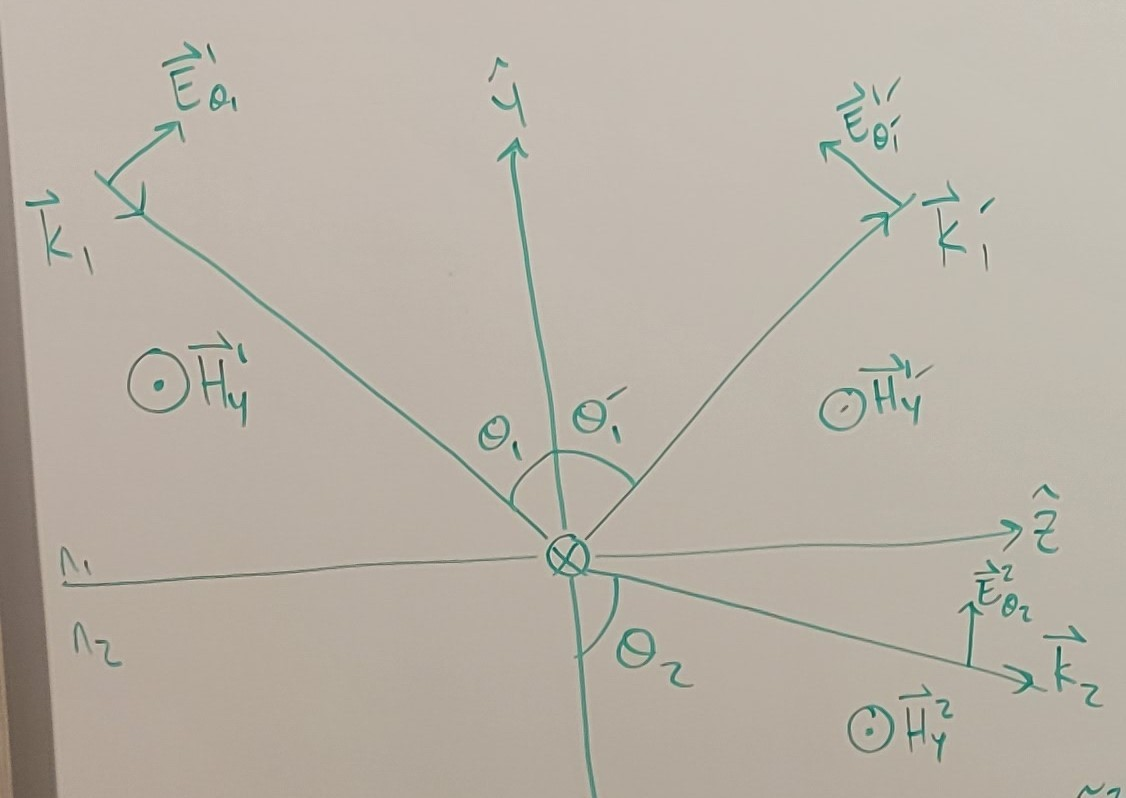
\includegraphics[width=0.8\textwidth]{TMG.jpg}
    \caption{Transverse Magnetic Geometry}
    \label{fig:my_label}
\end{figure}
Start with the general solutions:
\begin{align}
\vec{H}_{y}^{1} = \tilde{H}_{y}^{1} e^{\left( -i \vec{k}_{1} \cdot \vec{r}_{1} \right)} e^ {\left(-i \omega t \right)}; \quad 
\vec{k}_{1} = n_{1} \frac{\omega}{c_{1}} 
\begin{pmatrix}
	cos{\theta_{1}} \\
	sin{\theta_{1}}
\end{pmatrix}; \quad
\vec{r}_{1} = 
\begin{pmatrix}
	-x \\
	z
\end{pmatrix}
\end{align}
\begin{align}
\vec{H}_{y}^{1'} = \tilde{H}_{y}^{1'} e^{\left( -i \vec{k}_{1}^{'} \cdot \vec{r}_{1}^{'} \right)} e^ {\left(-i \omega t \right)}; \quad 
\vec{k}_{1}^{'} = n_{1} \frac{\omega}{c_{1}} 
\begin{pmatrix}
	-cos{\theta_{1}^{'}}\\
	sin{\theta_{1}^{'}}
\end{pmatrix}; \quad
\vec{r}_{1}^{'} = 
\begin{pmatrix}
	-x \\
	z
\end{pmatrix}
\end{align}
\begin{align}
\vec{H}_{y}^{2} = \tilde{H}_{y}^{2} e^{\left( -i \vec{k}_{2} \cdot \vec{r}_{2} \right)} e^ {\left(-i \omega t \right)}; \quad 
\vec{k}_{2} = n_{2} \frac{\omega}{c_{2}} 
\begin{pmatrix}
	cos{\theta_{2}} \\
	sin{\theta_{2}}
\end{pmatrix}; \quad
\vec{r}_{2} = 
\begin{pmatrix}
	-x \\
	z
\end{pmatrix}
\end{align}
Our boundary condition states that components $\vec{B}$ and $\vec{E}$ parallel to the interface are continuous. $\therefore$ $\vec{H}_{y}^{2} = \vec{H}_{y}^{1} + \vec{H}_{y}^{1'}$ at $x = 0$. \\

$e^ {\left(-i \omega t \right)}$ appear in each term and can be divided out of the equation, allowing us to write:
\begin{align}
\tilde{H}_{y}^{2} e^{\left( -i \vec{k}_{2} \cdot \vec{r}_{2} \right)} = \tilde{H}_{y}^{1} e^{\left( -i \vec{k}_{1} \cdot \vec{r}_{1} \right)} + \tilde{H}_{y}^{1'} e^{\left( -i \vec{k}_{1}^{'} \cdot \vec{r}_{1}^{'} \right)}
\end{align}
\begin{align}
\tilde{H}_{y}^{2} e^{\left( -i n_{2} \frac{\omega}{c_2} \cdot \begin{pmatrix}
	cos{\theta_{2}} \\
	sin{\theta_{2}}
\end{pmatrix} \cdot \begin{pmatrix}
	-x \\
	z
\end{pmatrix}
\right)} = \tilde{H}_{y}^{1} e^{\left( -i n_{1} \frac{\omega}{c_1} \cdot \begin{pmatrix}
	cos{\theta_{1}} \\
	sin{\theta_{1}} 
\end{pmatrix} \cdot \begin{pmatrix}
	-x \\
	z
\end{pmatrix}\right)} + \tilde{H}_{y}^{1'} e^{\left( -i n_{1} \cdot \begin{pmatrix}
	-cos{\theta_{1}^{'}} \\
	sin{\theta_{1}^{'}} 
\end{pmatrix} \cdot \begin{pmatrix}
	-x \\
	z
\end{pmatrix}
\right)}
\end{align}

Realize that $x = 0$, and $\theta_{1}^{'} = \theta_{1}$ and we can write:

\begin{align}
\tilde{H}_{y}^{2} e^{\left( -i n_{2} \frac{\omega}{c_2} z \sin{\theta}_{2}
\right)}  = \left(\tilde{H}_{y}^{1} + \tilde{H}_{y}^{1'} \right) e^{\left( -i n_{1} \frac{\omega}{c_1} z \sin{\theta}_{1}
\right)} 
\end{align}

Divide both sides by $\tilde{H}_{2}$ and take the natural logarithm:

\begin{align}
\left( -i n_{2} \frac{\omega}{c_2} z \sin{\theta}_{2}
\right)  =  \left( -i n_{1} \frac{\omega}{c_1} z \sin{\theta}_{1}
\right) 
\end{align}

Now divide through by $-i \omega z$ and we have our solution:

\begin{align}
\frac{n_2}{c_2} \sin{\theta}_{2} = \frac{n_1}{c_1} \sin{\theta}_{1}
\end{align}

\end{document}



























